% Template for Elsevier submission with R Markdown

% Stuff changed from PLOS Template
\documentclass[authoryear, review]{elsarticle}
\usepackage[american]{babel}
\usepackage[section]{placeins}

\bibliographystyle{model5-names}

\journal{Cognitive Psychology}



% amsmath package, useful for mathematical formulas
\usepackage{amsmath}
% amssymb package, useful for mathematical symbols
\usepackage{amssymb}

% hyperref package, useful for hyperlinks
\usepackage{hyperref}

% graphicx package, useful for including eps and pdf graphics
% include graphics with the command \includegraphics
\usepackage{graphicx}

% Sweave(-like)
\usepackage{fancyvrb}
\DefineVerbatimEnvironment{Sinput}{Verbatim}{fontshape=sl}
\DefineVerbatimEnvironment{Soutput}{Verbatim}{}
\DefineVerbatimEnvironment{Scode}{Verbatim}{fontshape=sl}
\newenvironment{Schunk}{}{}
\DefineVerbatimEnvironment{Code}{Verbatim}{}
\DefineVerbatimEnvironment{CodeInput}{Verbatim}{fontshape=sl}
\DefineVerbatimEnvironment{CodeOutput}{Verbatim}{}
\newenvironment{CodeChunk}{}{}

% cite package, to clean up citations in the main text. Do not remove.
\usepackage{cite}

\usepackage{color}

% Use doublespacing - comment out for single spacing
%\usepackage{setspace}
%\doublespacing

% % Text layout
\topmargin 0.0cm
\oddsidemargin 0.5cm
\evensidemargin 0.5cm
\textwidth 15cm
\textheight 21cm

% Bold the 'Figure #' in the caption and separate it with a period
% Captions will be left justified
\usepackage[labelfont=bf,labelsep=period,justification=raggedright]{caption}


% Remove brackets from numbering in List of References
\makeatletter
\renewcommand{\@biblabel}[1]{\quad#1.}
\makeatother


% Leave date blank
\date{}

\begin{document}

\begin{frontmatter}

\title{Social cues modulate the representations underlying cross-situational
learning}

\author[km]{\corref{cor}Kyle MacDonald}
\cortext[cor]{Corresponding author}
\ead{kyle.macdonald@stanford.edu}
\author[dy]{Daniel Yurovsky}
\author[mcf]{Michael C. Frank}
\address{Department of Psychology, Stanford University, United States}


\begin{abstract}
Because children hear language in environments that contain many things
to talk about, learning the meaning of even the simplest word requires
making inferences under uncertainty. A cross-situational statistical
learner can aggregate across naming events to form stable word-referent
mappings, but this approach neglects an important source of information
that can reduce referential uncertainty: social cues from speakers
(e.g., eye gaze). In four large-scale experiments with adults, we tested
the effects of varying referential uncertainty in cross-situational word
learning using social cues. Social cues shifted learners away from
tracking multiple hypotheses and towards storing only a single
hypothesis (Experiments 1 and 2). In addition, learners were sensitive
to graded changes in the strength of a social cue, and when it became
less reliable, they were more likely to store multiple hypotheses
(Experiment 3). Finally, learners stored fewer word-referent mappings in
the presence of a social cue even when visual inspection time was
equivalent to naming events without a social cue present (Experiment 4).
Taken together, our data suggest that the representations underlying
cross-situational word learning are quite flexible: In conditions of
greater uncertainty, learners store a broader range of information.
\end{abstract}

\begin{keyword}
statistical learning, social cues, word learning, language acquisition
\end{keyword}

\end{frontmatter}

\newpage

\section{Introduction}\label{introduction}

Learning the meaning of a new word should be hard. Consider that even
concrete nouns are often used in complex contexts with multiple possible
referents, which in turn have many conceptually natural properties that
a speaker could talk about. This ambiguity creates the potential for an
(in principle) unlimited amount of referential uncertainty in the
learning task.\footnote{This problem is a simplified version of Quine's
  \textit{indeterminacy of reference} (Quine, 1960): That there are many
  possible meanings for a word (``Gavigai'') that include the referent
  (``Rabbit'') in their extension, e.g., ``white,'' ``rabbit,''
  ``dinner.'' Quine's broader philosophical point was that different
  meanings (``rabbit'' and ``undetached rabbit parts'') could actually
  be extensionally identical and thus impossible to tease apart.}
Remarkably, word learning proceeds despite this uncertainty, with
estimates of adult vocabularies ranging between 50,000 to 100,000
distinct words (P. Bloom, 2002). How do learners infer and retain such a
large variety of word meanings from data with this kind of ambiguity?

Statistical learning theories offer a solution to this problem by
aggregating cross-situational statistics across labeling events to
identify underlying word meanings (Siskind, 1996; Yu \& Smith, 2007).
Recent experimental has shown that both adults and young infants can use
word-object co-occurrence statistics to learn words from individually
ambiguous naming events (Smith \& Yu, 2008; Vouloumanos, 2008). For
example, Smith and Yu (2008) taught 12-month-olds three novel words
simply by repeating consistent novel word-object pairings across 10
ambiguous exposure trials. Moreover, computational models suggest that
cross-situational learning can scale up to learn adult-sized lexicons,
even under conditions of considerable referential uncertainty (K. Smith,
Smith, \& Blythe, 2011).

Although all cross-situational learning models agree that the input is
the co-occurrence between words and objects and the output is stable
word-object mappings, they disagree about how closely learners
approximate the input distribution (for review, see Smith, Suanda, \& Yu
2014). One approach has been to model learning as a process of updating
connection strengths between multiple word-object links (McMurray,
Horst, \& Samuelson, 2012), while other approaches have argued that
learners store only a single word-object hypothesis (Trueswell, Medina,
Hafri, \& Gleitman, 2013). In recent experimental and modeling work,
Yurovsky and Frank (2015) have suggested an integrative explanation
where learners allocate a fixed amount of attention to a single
hypothesis, and distribute the rest evenly among the remaining
alternatives. As the set of alternatives grows, the amount of attention
allocated to each object approaches zero.

In addition to the debate about representation, researchers also
disagree about how to characterize the ambiguity of the input to
cross-situational learning mechanisms. One way to quantify the
uncertainty in a naming event is to show adults video clips of
caregiver-child interactions and ask them to guess the meaning of an
intended referent (Human Simulation Paradigm: HSP). Using the HSP,
Medina, Snedeker, Trueswell, and Gleitman (2011) found that
approximately 90\% of learning episodes were ambiguous (\textless{} 33\%
accuracy) and 7\% were relatively unambiguous (\textgreater{} 50\%
accuracy). In contrast, Yurovsky, Smith, and Yu (2013) found more of a
bimodal distribution of referential uncertainty, with approximately 20\%
of naming events being ambiguous (\textless{} 10\% accuracy) and 30\%
being unambiguous (\textgreater{} 90\% accuracy). Cartmill, Armstrong,
Gleitman, Goldin-Meadow, Medina, and Trueswell (2013) also showed that
the proportion of unambiguous naming episodes varies across parents,
with some parents rarely providing highly informative contexts and
others' doing so relatively more often.\footnote{Note that the different
  estimates of referential uncertainty in these studies could be driven
  by the different sampling procedures used to select naming events for
  the HSP. Yurovsky, Smith, and Yu (2013) sampled utterances for which
  the parent labeled a co-present object, whereas Medina, Snedeker,
  Trueswell, et al. (2011) randomly sampled any utterances containing
  concrete nouns. Regardless of these differences, the key point here is
  that variability in referential uncertainty across naming events
  exists and can alter the representations underlying cross-situational
  learning.}

Thus, representations in cross-situational word learning can appear
distributional or discrete, and the input to statistical learning
mechanisms can vary along a continuum from low to high ambiguity. These
results raise an interesting question: could learners be sensitive to
the ambiguity of the input and use this information to flexibly alter
the representations they store in memory? In the current line of work,
we investigated how the presence of referential cues in the social
context might alter the ambiguity of the input to statistical word
learning mechanisms.

Social-pragmatic theories of language acquisition emphasize the
importance of social cues for word learning (P. Bloom, 2002; Clark,
2009; Hollich et al., 2000). Experimental work has shown that even
children as young as 16 months are sophisticated intention-readers,
preferring to map novel words to objects that are the target of a
speaker's gaze and not their own (Baldwin, 1993). In an analysis of
naturalistic parent-child labeling events, Yu and Smith (2012) {]}
showed that young learners tended to retain labels that were accompanied
with clear referential cues that were concurrent with visual access. And
correlational data has shown strong links between early
intention-reading skills (e.g., gaze following) and later vocabulary
growth (Brooks \& Meltzoff, 2005, 2008; Carpenter, Nagell, Tomasello,
Butterworth, \& Moore, 1998). Moreover, studies outside the domain of
language acquisition have shown that the presence of social cues: (a)
produced better spatial learning of audiovisual events (Wu, Gopnik,
Richardson, \& Kirkham, 2011), (b) boosted recognition of a cued object
(Cleveland, Schug, \& Striano, 2007), and (c) lead to preferential
encoding of an object's featural information (Yoon, Johnson, \& Csibra,
2008). Together, the evidence suggests that social cues could alter the
representations stored during cross-situational word learning by
modulating how people allocate attention to the relevant statistics in
the input.

The goal of the current study is to ask whether the presence of a valid
social cue, a speaker's gaze, can change the representations underlying
cross-situational word learning. We used a modified version of Yurovsky
and Frank (2015)'s paradigm to provide a direct measure of memory for
alternative word-object links during cross-situational learning. In
Experiment 1, we manipulated the presence of a referential cue at
different levels of attention and memory demands. At all levels of
difficulty, learners tracked a strong single hypothesis but were less
likely to track multiple word-object links when a social cue was
present. In Experiment 2, we replicated the findings from Experiment 1
using a more ecologically valid social cue. In Experiment 3, we moved to
a parametric manipulation of referential uncertainty by varying the
reliability of the speaker's gaze. Learners were sensitive to graded
changes in reliability and retained more word-object links as
uncertainty in the input increased. Finally, in Experiment 4, we fixed
the length of the initial naming events across the gaze and no-gaze
conditions. Learners stored less information in the presence of gaze
despite even when they had visually inspected the objects for the same
amount of time. In sum, our data suggest that cross-situational word
learners are quite flexible, storing representations with different
levels of fidelity depending on the amount of ambiguity present during
learning.

\section{Experiment 1}\label{experiment-1}

We set out to test the effect of a referential cue on the
representations underlying cross-situational word learning. We used a
version of Yurovsky and Frank (2015)'s paradigm where we manipulated the
ambiguity of the learning context by including a gaze cue from a
schematic, female interlocutor. Participants saw a series of ambiguous
exposure trials where they heard one novel word that was either paired
with a gaze cue or not and selected the object they thought went with
each word. In subsequent test trials, participants heard the novel word
again, this time, paired with a new set of novel objects. One of the
objects in this set was either the participant's initial guess (Same
test trials) or one of the objects was \emph{not} their initial guess
(Switch test trials). Performance on Switch trials provided a direct
measure of whether referential cues influenced the number of alternative
word-object links that learners stored in memory. If learners performed
worse on Switch trials after an exposure trial with gaze, this suggests
that they stored fewer additional objects from the initial learning
context.

\subsection{Method}\label{method}

\subsubsection{Participants}\label{participants}

We posted a set of Human Intelligence Tasks (HITs) to Amazon Mechanical
Turk. Only participants with US IP addresses and a task approval rate
above 95\% were allowed to participate, and each HIT paid 30 cents.
50-100 HITs were posted for each of the 32 between-subjects conditions.
Data were excluded if participants completed the task more than once or
if participants did not respond correctly on familiar object trials (131
HITs). The final sample consisted of 1438 participants.

\begin{CodeChunk}
\begin{figure}[tb]

{\centering 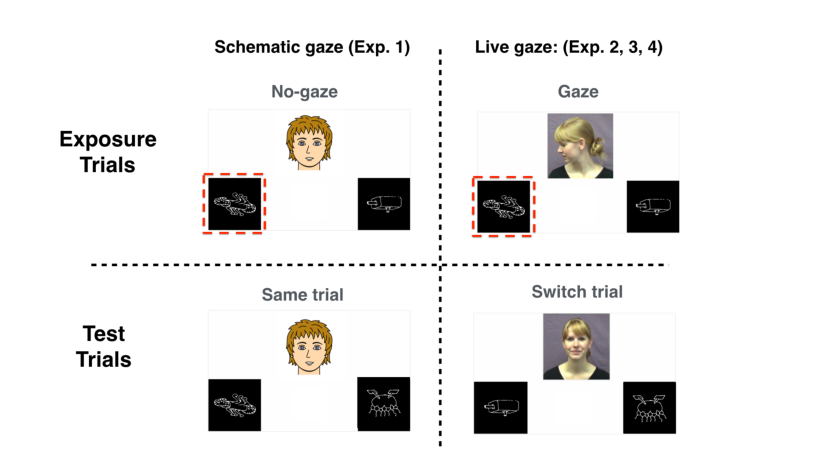
\includegraphics[width=1\linewidth]{figs/stimuli-1} 

}

\caption[Screenshots of exposure and test trials from Experiment 1 (schematic gaze cue) and Experiments 2, 3 \& 4 (human actress gaze cue)]{Screenshots of exposure and test trials from Experiment 1 (schematic gaze cue) and Experiments 2, 3 \& 4 (human actress gaze cue). Participants saw exposure trials with or without a gaze cue depending on condition assignment. All participants saw both types of test trials: Same and Switch. On Same trials, the object that participants chose during exposure appeared with a new novel object. On Switch trials the object that participants did not choose appeared with a new novel object. Participants saw either 2, 4, 6, or 8 referents depending on their condition assignment.}\label{fig:stimuli}
\end{figure}
\end{CodeChunk}

\subsubsection{Stimuli}\label{stimuli}

Figure 1 shows screenshots taken from Experiment 1. Visual stimuli were
black and white pictures of familiar and novel objects taken from
Kanwisher, Woods, Iacoboni, and Mazziotta (1997). Auditory stimuli were
recordings of familiar and novel words by an AT\&T Natural Voices
\texttrademark (voice: Crystal) speech synthesizer. Novel words were 1-3
syllable pseudowords that obeyed all rules of English phonotactics. A
schematic drawing of a human speaker was chosen for ease of manipulating
the direction of gaze, the referential cue of interest in this study.
All experiments can be viewed and downloaded at the project page:
\url{https://kemacdonald.github.io/soc_xsit/}.

\subsubsection{Design and Procedure}\label{design-and-procedure}

Participants saw a total of 16 trials: eight exposure trials and eight
test trials. On each trial, they heard one novel word, saw a set of
novel objects, and were asked to guess which object went with the word.
Before seeing exposure and test trials, participants completed four
practice trials with familiar words and objects. These trials
familiarized participants to the task and allowed us to exclude
participants who were unlikely to perform the task as directed either
because of inattention or because their computer audio was turned off.

After the practice trials, participants were told that they would now
hear novel words and see novel objects and that their task was to select
the referent that ``goes with each word.'' Over the course of the
experiment, participants heard eight novel words two times, with one
exposure trial and one test trial for each word. Four of the test trials
were \emph{Same} trials in which the object that participants selected
on the exposure trial was shown with a set of new novel objects. The
other four test trials were \emph{Switch} trials in which one of the
objects was chosen at random from the set of objects that the
participant did not select on exposure.

Participants were randomly assigned to one of the 32 between-subjects
conditions (4 Referents X 4 Intervals X 2 Gaze conditions). Participants
either saw 2, 4, 6, or 8 referents on the screen and test trials
occurred at different intervals after exposure trials: either 0, 1, 3,
or 7 trials from the initial exposure to a word. For example, in the
0-interval condition, the test trial for that word would occur
immediately following the exposure trial, but in the 3-interval
condition, participants would see three additional exposure trials for
other novel words before seeing the test trial for the initial word. The
interval conditions modulated the time delay between learning and test,
and the number of referents conditions modulated the attention demands
present during learning.

Participants were assigned to either the Gaze or No-Gaze condition. In
the Gaze condition, gaze was directed towards one of the objects on
exposure trials; in the No-Gaze condition, gaze was always directed
straight ahead (see Figure 1 for examples). At test, gaze was always
directed straight ahead. To show participants that their response had
been recorded, a red box appeared around the selected object for one
second. This box always appeared around the selected object, even if
participants' selections were incorrect.

\subsection{Results and Discussion}\label{results-and-discussion}

\subsubsection{Analysis plan}\label{analysis-plan}

The structure of our analysis plan is parallel across all four
experiments. First, we examined accuracy and response time on exposure
trials to provide evidence that learners were (a) sensitive to our
experimental manipulation and (b) altered their allocation of attention
in response to the presence of a social cue. Accuracy on exposure trials
was defined as selecting the referent that was the target of gaze in the
Gaze condition (note that there was no ``correct'' behavior for exposure
trials in the No-Gaze condition). Next, we examined accuracy on test
trials to test whether learners' memory for alternative word-object
links changed depending on the ambiguity of the learning context.
Accuracy on test trials (both Same and Switch) was defined as selecting
the referent that was present during the exposure trial for that word.

The key behavioral prediction of our hypothesis is that the presence of
gaze would result in reduced memory for multiple word-object links,
operationalized as a decrease in accuracy on Switch test trials after
seeing exposure trials with a gaze cue. To quantify participants'
behavior, we used mixed-effects regression models with the maximal
random effects structure justified by our experimental design:
by-subject intercepts and slopes for each trial type. We limited all
models to include only two-way interactions because the critical test of
our hypothesis was the interaction between gaze condition and trial
type, and we did not have theoretical predictions for any possible
three-way or four-way interactions. All models were fit using the lme4
package in R (Bates, Maechler, Bolker, \& Walker, 2013), and all of our
data and our processing/analysis code can be viewed in the version
control repository for this paper at:
\url{https://github.com/kemacdonald/soc_xsit}.

\begin{CodeChunk}
\begin{figure}[tb]

{\centering 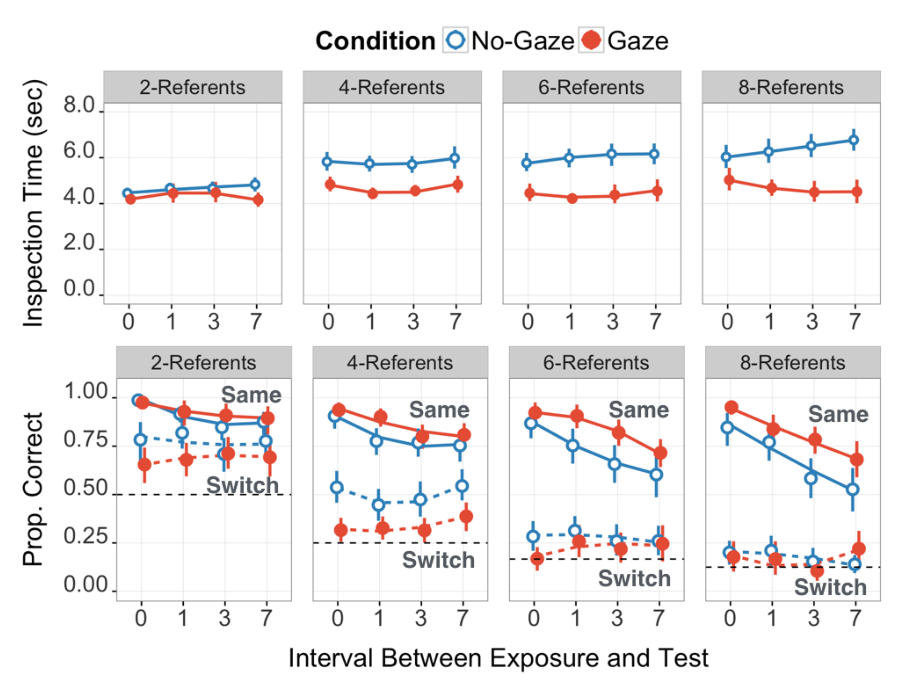
\includegraphics[width=1\linewidth]{figs/expt1-plot-1} 

}

\caption[Experiment 1 results]{Experiment 1 results. The top row shows average inspection times on exposure trials for all experimental conditions as a function of the number of trials that occurred between exposure and test. Each panel represents a different number of referents, and line color represents the Gaze and No-Gaze conditions. The bottom row shows accuracy on test trials for all conditions as a function of the number of intervening trials. The horizontal dashed lines represent chance performance for each number of referents, and the type of line (solid vs. dashed) represents the different test trial types (Same vs. Switch). Error bars indicate 95\% confidence intervals computed by non-parametric bootstrap.}\label{fig:expt1-plot}
\end{figure}
\end{CodeChunk}

\subsubsection{Exposure trials}\label{exposure-trials}

To ensure that our referential cue manipulation was effective, we
compared participants' accuracies on exposure trials in the Gaze
condition to a model of random behavior defined as a Binomial
distribution with a probability of success \(\frac{1}{Num Referents}\).
Correct performance was defined as selecting the object that was the
target of the speaker's gaze. Following Yurovsky and Frank (2015), we
fit logistic regressions for each gaze, referent, and interval
combination specified as
\texttt{Gaze Target $\sim$ 1 + offset(logit(1/Referents))}. The offset
encoded the chance probability of success given the number of referents,
and the coefficient for the intercept term shows on a log-odds scale how
much more likely participants were to select the gaze target than would
be expected if participants were selecting randomly. In all conditions,
participants used gaze to select referents on exposure trials more often
than expected by chance (smallest \(\beta\) = 1.4, z = 9.38, \(p\)
\textless{} .001). However, there was variability across conditions in
the mean proportion of gaze cue (overall \(M\) = 0.84, smallest \(M\) =
0.77, largest \(M\) = 0.93).

We were also interested in differences in participants' response times
across the experimental conditions. Since these trials were self-paced,
participants could choose how much time to spend inspecting the
referents on the screen, thus providing an index of participants'
attention. To quantify the effects of gaze, interval, and number of
referents, we fit a linear mixed-effects model that predicted
participants' inspection times as follows:
\texttt{Log(Inspection time) $\sim$ Gaze * Log(Interval) + Gaze * Log(Referents) + (1 | subject)}.
We found a significant main effect of the number of referents (\(\beta\)
= 0.34, p \textless{} .001) with longer inspection times as the number
of referents increased, a significant two-way interaction between gaze
condition and the number of referents (\(\beta\) = -0.27, p \textless{}
.001) with longer inspection times in the No-Gaze condition, especially
as the number of referents increased, and a significant two-way
interaction between gaze condition and interval (\(\beta\) = -0.08,
\(p\) = 0.004) with slower inspection times in the No-Gaze condition,
especially as the number of intervening trials increased (see the top
row of Figure 2). Shorter inspection times on exposure trials with gaze
provides evidence that the presence of a referential cue focused
participants' attention on a single referent and away from alternative
word-object links.

\subsubsection{Test trials}\label{test-trials}

Next, we explored participants' accuracy in identifying the referent for
each word in all conditions for both kinds of test trials (see the
bottom row of Figure 2). We first compared the distribution of correct
responses made by each participant to the distribution expected if
participants were selecting randomly defined as a Binomial distribution
with a probability of success \(\frac{1}{Num Referents}\). Correct
performance is defined as selecting the object that was present on the
exposure trial for that word. We fit the same logistic regressions as we
did for exposure trials:
\texttt{Correct $\sim$ 1 + offset(logit(1/Referents))}. In 31 out of the
32 conditions for both Same and Switch trials, participants chose the
correct object more often than would be expected by chance (smallest
\(\beta\) = 0.36, \(z\) = 2.44, \(p\) = 0.01). On Switch trials in the
8-referent, 3-interval condition, participants' responses were not
significantly different from chance (\(\beta\) = 0.06, z = 0.33, p =
0.74). Participants' success on Switch trials replicates the findings
from Yurovsky and Frank (2015) and provides direct evidence that
learners encode more than a single hypothesis in ambiguous word learning
situations even under high attentional and memory demands and in the
presence of a referential cue.

\begin{table}[tb]
\centering
\begin{tabular}{lrrrrl}
 Predictor & Estimate & Std. Error & $z$ value & $p$ value &  \\ 
  \hline
Intercept & 3.01 & 0.29 & 10.35 & $<$ .001 & *** \\ 
  Switch Trial & -1.36 & 0.24 & -5.63 & $<$ .001 & *** \\ 
  Gaze Condition & 0.12 & 0.26 & 0.47 & 0.64 &  \\ 
  Log(Interval) & -0.45 & 0.11 & -4.08 & $<$ .001 & *** \\ 
  Log(Referents) & 0.23 & 0.11 & 2.02 & 0.04 & * \\ 
  Switch Trial*Gaze Condition & -1.09 & 0.12 & -9.07 & $<$ .001 & *** \\ 
  Switch Trial*Log(Interval) & 0.52 & 0.05 & 9.50 & $<$ .001 & *** \\ 
  Switch Trial*Log(Referent) & -0.59 & 0.09 & -6.49 & $<$ .001 & *** \\ 
  Gaze Condition*Log(Interval) & 0.06 & 0.06 & 1.00 & 0.32 &  \\ 
  Gaze Condition*Log(Referent) & 0.20 & 0.09 & 2.15 & 0.03 & * \\ 
  Log(Interval)*Log(Referent) & -0.04 & 0.04 & -1.02 & 0.31 &  \\ 
   \hline
\end{tabular}
\caption{Predictor estimates with standard errors and significance information for a logistic mixed-effects model predicting word learning in Experiment 1.} 
\label{tab:exp1_reg}
\end{table}

To quantify the effects of gaze, interval, and number of referents on
the probability of a correct response, we fit the following
mixed-effects logistic regression model to a filtered dataset where we
removed participants who did not reliably select the object that was the
target of gaze on exposure trials:\footnote{We did not predict that
  there would be a subset of participants who would not follow the gaze
  cue, thus this filtering criteria was developed posthoc. However, we
  think that the filter is theoretically motivated because we would only
  expect to see an effect of gaze if participants actually used the gaze
  cue. The filter removed 94 participants (6\% of the sample). The key
  inferences from the data do not depend on this filtering criteria.}
\texttt{Correct $\sim$ Trial Type * Gaze + Trial Type * Log(Interval) + Trial Type * \\ Log(Referents) + offset(logit($^1/_{Referents}$)) + (TrialType | subject)}.

We coded interval and number of referents as continuous predictors and
transformed these variables to the log scale. We limited the model to
include only two-way interactions because the critical test of our
hypothesis is the interaction between gaze condition and trial type, and
we did not have any theoretical predictions for possible three-way
interactions.
\footnote{If we allowed for three-way interactions in the model, there was a marginally significant interaction between gaze condition, trial type, and interval ($\beta = 0.21$, $p$ = 0.058). The two-way interaction between gaze condition and trial type remained significant in this more complex model ($\beta = -1.3$, $p$ = 0.006). A model including four-way interactions did not sufficiently improve model fit in order to justify the added complexity.}

Table 1 shows the output of the logistic regression. We found
significant main effects of the number of referents (\(\beta = 0.23\), p
\textless{} .001) and interval (\(\beta = -0.45\), p \textless{} .001),
such that as each of these factors increased, accuracy on test trials
decreased. We also found a significant main effect of trial type
(\(\beta = -1.36\), p \textless{} .001), with worse performance on
Switch trials. There were significant interactions between trial type
and interval (\(\beta = 0.52\), p \textless{} .001), trial type and
referents (\(\beta = -0.59\), p \textless{} .001), and gaze condition
and referents (\(\beta = 0.2\), p \textless{} .05). These interactions
can be interpreted as meaning: (a) the interval between exposure and
test affected Same trials more than Switch trials, (b) the number of
referents affected Switch trials more than Same trials, and (c)
participants performed slightly better at the higher number of referents
in the Gaze condition. The interactions between gaze condition and
referents and between referents and interval were not significant.
Importantly, we found the predicted interaction between trial type and
gaze condition (\(\beta = -1.09\), p \textless{} .001), with
participants in the Gaze condition performing worse on Switch trials.
This interaction provides direct evidence that the presence of a
referential cue selectively reduces participants' memory for alternative
word-object links.

We were also interested in how inspection times on exposure trials would
affect participants' accuracy at test. So we fit an additional model
where participants' inspection times were added as a predictor. We found
a significant interaction between inspection time and gaze condition
(\(\beta = -0.17\), \(p\) = 0.01), such that longer inspection times
provided a larger boost to accuracy in the No-Gaze condition. This
interaction suggests that the presence of a referential cue modulated
the relationship between attention on exposure trials and memory at
test. Importantly, the key test of our hypothesis, the interaction
between gaze condition and trial type, remained significant in this
alternative version of the model (\(\beta\) = -1.02, \(p\) = p
\textless{} .001).

Taken together, the inspection time and accuracy analyses provide
evidence that the presence of a referential cue modulated learners'
attention during learning, and in turn made them less likely to track
multiple word-object links. We did not see strong evidence that reduced
tracking of alternatives resulted in an increase in performance on Same
trials. This finding suggests that the limitations on Same trials may be
different than those regulating the distribution of attention on Switch
trials since the presence of a referential cue selectively reduced
learners tracking of alternatives but apparently did not lead learners
to form a stronger memory of their single candidate hypothesis.

There was relatively large variation in performance across conditions in
group-level accuracy scores and in participants' tendency to \emph{use}
the referential cue on exposure trials. Moreover, we found a subset of
participants who did not reliably use the gaze cue at all, potentially
reducing the effect of gaze on cross-situational learning in this
experiment. It is possible that the effect of gaze was reduced because
the referential cue that we used -- a static schematic drawing of a
speaker -- was relatively weak compared to the cues present in
real-world learning environments. Thus we do not yet know how learners'
memory for alternatives during cross-situational learning would change
in the presence of a stronger and more ecologically valid referential
cue. We designed Experiment 2 to address this question.

\section{Experiment 2}\label{experiment-2}

In Experiment 2, we set out to replicate the findings from Experiment 1
using a more ecologically valid stimulus set. We replaced the static,
schematic drawing with a video of a live actress. While the video
stimuli were still far from actual learning contexts, it included a real
person who provided both a gaze cue and a head turn towards the target
object. To reduce the across-conditions variability that we found in
Experiment 1, we introduced a within-subjects design where each
participant saw both Gaze and No-Gaze exposure trials in a blocked
design. We selected a subset of the conditions from Experiment 1 and
tested only the 4-referent display with 0 and 3 intervening trials as
between-subjects manipulations. Our goals were to replicate the
reduction in learners' tracking of alternative word-object links in the
presence of a referential cue and to test whether increasing the
ecological validity of the cue would result in a boost to the strength
of learners' recall of their candidate hypothesis.

\subsection{Method}\label{method-1}

\subsubsection{Participants}\label{participants-1}

Participant recruitment and inclusionary/exclusionary criteria were
identical to those of Experiment 1. 100 HITs were posted for each
condition (1 Referent X 2 Intervals X 2 Gaze conditions) for total of
400 paid HITs (excluded 33 HITs).

\subsubsection{Stimuli}\label{stimuli-1}

Audio and picture stimuli were identical to Experiment 1. The
referential cue in the Gaze condition was a video (see Figure 1). On
each exposure trial, the actress looked out at the participant with a
neutral expression, smiled, and then turned to look at one of the four
images on the screen. She maintained her gaze for 3 seconds before
returning to the center. On test trials, she looked straight ahead for
the duration of the trial.

\subsection{Design and Procedure}\label{design-and-procedure-1}

Procedures were identical to those of Experiment 1. The major design
change was a within-subjects manipulation of the gaze cue where each
participant saw exposure trials with and without gaze. The experiment
consisted of 32 trials broken down into 2 blocks of 16 trials. Each
block consisted of 8 exposure trials and 8 test trials (4 Same trials
and 4 Switch trials) and contained only Gaze or No-gaze exposure trials.
The order of block was counterbalanced across participants.

\subsection{Results and Discussion}\label{results-and-discussion-1}

We followed the same analysis plan as in Experiment 1. We first analyzed
inspection times and accuracy on exposure trials and then analyzed
accuracy on test trials.

\subsubsection{Exposure trials}\label{exposure-trials-1}

Similar to Experiment 1, participants' responses on exposure trials
differed from those expected by chance (smallest \(\beta\) = 3.42, z =
33.43, p \textless{} .001), suggesting that gaze was effective in
directing participants' attention. Participants in Experiment 2 were
more consistent in their use of gaze with the live action stimuli
compared to the schematic stimuli used in Experiment 1 (\(M_{Exp1}\) =
0.8, \(M_{Exp2}\) = 0.91\$), suggesting that using a live actress
increased participants' willingness to use the gaze cue.

We replicated the findings from Experiment 1. Inspection times were
shorter in the Gaze (\(\beta\) = -1.11, p \textless{} .001) and the
3-interval condition (\(\beta\) = -0.5, p \textless{} .001). The
interaction between gaze and interval was not significant, meaning that
gaze had the same effect on participants' inspection times at both
intervals (see Panel A of Figure 3).

\begin{CodeChunk}
\begin{figure}[tb]

{\centering 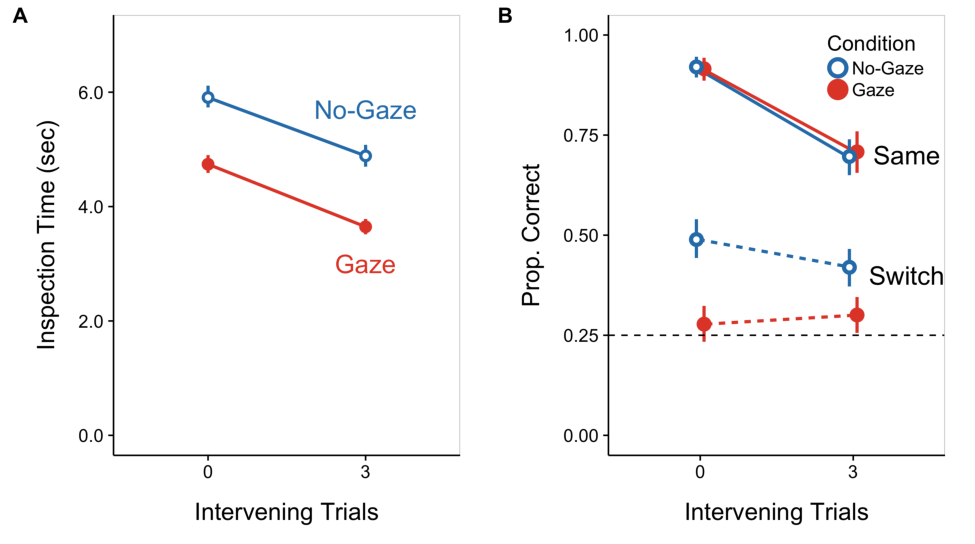
\includegraphics[width=1\linewidth]{figs/expt2-plot-1} 

}

\caption[Experiment 2 results]{Experiment 2 results. Panel A shows inspection times on exposure trials as a function of interval and for trials with and without gaze. Panel B shows accuracy for Same and Switch test trials as a function of the number of intervening trials between exposure and test for trials with and without gaze. The dashed line in Panel B represents chance performance. Error bars indicate 95\% confidence intervals computed by non-parametric bootstrap.}\label{fig:expt2-plot}
\end{figure}
\end{CodeChunk}

\subsubsection{Test trials}\label{test-trials-1}

\begin{table}[tb]
\centering
\begin{tabular}{lrrrrl}
 Predictor & Estimate & Std. Error & $z$ value & $p$ value &  \\ 
  \hline
Intercept & 2.98 & 0.18 & 16.20 & $<$ .001 & *** \\ 
  Switch Trial & -3.04 & 0.18 & -16.47 & $<$ .001 & *** \\ 
  Gaze Condition & -0.15 & 0.16 & -0.98 & 0.33 &  \\ 
  Log(Interval) & -0.98 & 0.10 & -9.62 & $<$ .001 & *** \\ 
  Switch Trial*Gaze Condition & -0.65 & 0.15 & -4.32 & $<$ .001 & *** \\ 
  Switch Trial*Log(Interval) & 0.85 & 0.10 & 8.68 & $<$ .001 & *** \\ 
  Gaze Condition*Log(Interval) & 0.14 & 0.07 & 1.90 & 0.06 & . \\ 
   \hline
\end{tabular}
\caption{Predictor estimates with standard errors and significance information for a logistic mixed-effects model predicting word learning in Experiment 2.} 
\label{tab:exp2_reg}
\end{table}

Across all conditions for both trial types participants selected the
correct referent at rates greater than chance (smallest \(\beta\) =
0.58, z = 9.68, p \textless{} .001). We replicated the critical finding
from Experiment 1: after seeing exposure trials with gaze, participants
performed worse on Switch trials, meaning they stored fewer word-object
links (\(\beta = -0.65\), p \textless{}
.001).\footnote{As in Experiment 1, we fit this model to a filtered dataset removing participants who did not reliably use the gaze cue.}
Participants were also less accurate as the interval between exposure
and test increased (\(\beta\) = -0.98, p \textless{} .001) and on the
Switch trials overall (\(\beta = -3.04\), p \textless{} .001).

In addition, there was a significant two-way interaction between trial
type and interval (\(\beta = 0.85\), p \textless{} .001), with worse
performance on Switch trials in the 3-interval condition. The two-way
interaction between gaze condition and interval was marginally
significant (\(\beta = 0.14\), p = 0.057), such that participants in the
gaze condition were less affected by the increase in interval. Similar
to Experiment 1, we did not see evidence of a boost to performance on
Same trials in the gaze condition.

Next, we added inspection times on exposure trials as a predictor of
accuracy at test. We found a marginally significant main effect of
inspection time (\(\beta\) = 0.182, \(p\) = 0.096) with higher accuracy
as inspection time increased. Similar to Experiment 1, the interaction
between gaze and trial type remained significant even when inspection
time was added to the model (\(\beta\) = -0.547, \(p\) \textless{}
.001).

The results of Experiment 2 provide converging evidence for our
hypothesis, showing that the presence of a referential cue reliably
focuses learners' attention away from alternative word-object links and
shifts them towards single hypothesis tracking. Moving to a live action
stimulus led to higher rates of selecting the target of gaze on exposure
trials, but did not result in a boost to performance on Same trials. The
selective effect of gaze on Switch trials provides additional evidence
that the fidelity of participants' single hypothesis was unaffected by
the presence of a referential cue in our paradigm.

Thus far we have shown that people store different amounts of
information in response to a categorical manipulation of referential
uncertainty. In both Experiments 1 and 2, the learning context was
either entirely ambiguous (No-Gaze) or entirely unambiguous (Gaze). But
not all real-world learning contexts fall at the extremes of this
continuum (although see Yurovsky et al., 2013). Could learners be
sensitive to more subtle changes in the quality of learning contexts? In
our next experiment, we tested a prediction of our account: whether
learners would store more word-object links in response to graded
changes in referential uncertainty during learning.

\section{Experiment 3}\label{experiment-3}

In Experiment 3, we explored whether learners would allocate attention
and memory flexibly in response to \emph{graded} changes in the
referential uncertainty that was present during learning. To test this
hypothesis, we moved beyond a categorical manipulation of the
presence/absence of gaze, and we parametrically varied the strength of
the referential cue. We manipulated cue strength by adding a block of
familiarization trials where we varied the proportion of Same and Switch
trials. If participants saw more Switch trials, this provided evidence
that the speaker's gaze was a less reliable cue to reference. This
design was inspired by a growing body of experimental work showing that
even young children are sensitive to the prior reliability of speakers
and will use this information to decide whom to learn novel words from
(Koenig, Clement, \& Harris, 2004).

\subsection{Method}\label{method-2}

\subsubsection{Participants}\label{participants-2}

Participant recruitment and inclusionary/exclusionary criteria were
identical to those of Experiment 1 and 2 (excluded 27 HITs). 100 HITs
were posted for each reliability level (0\%, 25\%, 50\%, 75\%, and
100\%) for total of 500 paid HITs.

\subsubsection{Design and Procedure}\label{design-and-procedure-2}

Procedures were identical to those of Experiments 1 and 2. We modified
the design of our cross-situational learning paradigm to include a block
of 16 familiarization trials (8 exposure trials and 8 test trials) at
the beginning of the experiment. These trials served to establish the
reliability of the speaker's gaze. To establish reliability, we varied
the proportion of Same/Switch trials that occurred during the
familiarization block. Recall that on Switch trials the gaze target did
not show up at test, which provided evidence that the speaker's gaze was
not a reliable cue to reference. Reliability was a between-subjects
manipulation such that participants either saw 8, 6, 4, 2, or 0 Switch
trials during familiarization, which corresponded to the 0\%, 25\%,
50\%, 75\%, or 100\% reliability conditions. After the familiarization
block, participants completed another block of 16 trials (8 exposure
trials and 8 test trials). Since we were no longer testing the effect of
the presence or absence of a referential cue, all exposure trials
throughout the experiment included a gaze cue. Finally, at the end of
the task, we asked participants to assess the reliability of the speaker
on a continuous scale from ``completely unreliable'' to ``completely
reliable.''

\subsection{Results and Discussion}\label{results-and-discussion-2}

\subsubsection{Exposure trials}\label{exposure-trials-2}

Participants reliably chose the referent that was the target of gaze at
rates greater than chance (smallest \(\beta\) = 2.62, z = 33.43, p
\textless{} .001). We fit a mixed effects logistic regression model
predicting the probability of selecting the gaze target as follows:
\texttt{Correct-Exposure $\sim$ Reliability Condition * Subjective Reliability + (1 | subject)}.
We found an effect of reliability condition (\(\beta\) = 3.28, \(p\) =
0.03) such that when the gaze cue was more reliable, participants were
more likely to use it (\(M_{0\%}\) = 0.83, \(M_{25\%}\) = 0.82,
\(M_{50\%}\) = 0.87, \(M_{75\%}\) = 0.9, \(M_{100\%}\) = 0.94). We also
found an effect of subjective reliability (\(\beta\) = 7.26, p
\textless{} .001) such that when participants thought the gaze cue was
reliable, they were more likely to use it. The interaction between
reliability condition and subjective reliability assessments was
marginally significant (\(\beta\) = -4.58, \(p\)= 0.092). This analysis
provides evidence that participants were sensitive to the reliability
manipulation both in how often they used the gaze cue and in how they
rated the reliability of the speaker at the end of the task.

\subsubsection{Test trials}\label{test-trials-2}

\begin{CodeChunk}
\begin{figure}[tb]

{\centering 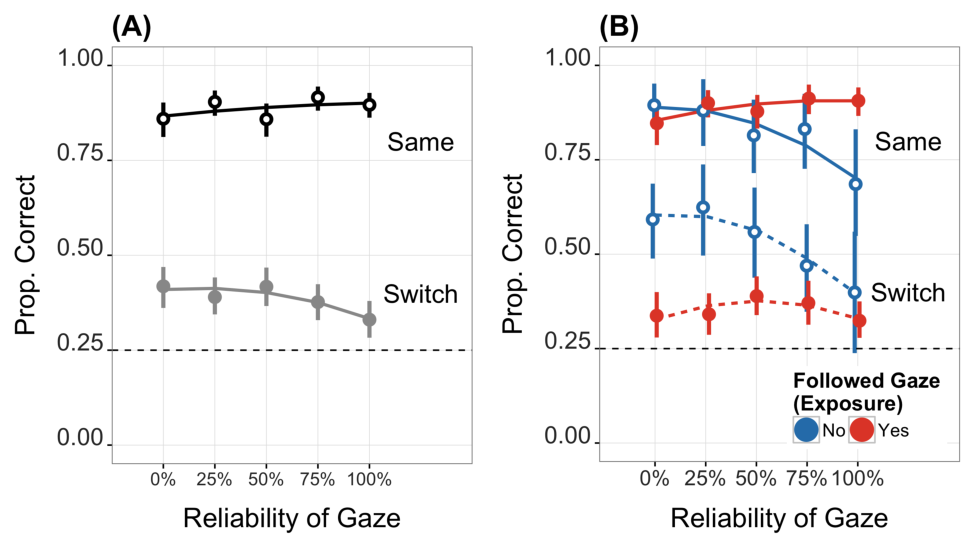
\includegraphics[width=0.9\linewidth]{figs/e3-plot-1} 

}

\caption[Primary analyses of test trial performance in Experiment 3]{Primary analyses of test trial performance in Experiment 3. Panel A shows performance as a function of reliability condition. Panel B shows performance as a function of reliability condition and whether participants chose to follow gaze on exposure trials. The horizontal dashed lines represent chance performance, and error bars indicate 95\% confidence intervals computed by non-parametric bootstrap.}\label{fig:e3-plot}
\end{figure}
\end{CodeChunk}

Next, we tested whether the reliability manipulation altered the
strength of participants' memory for alternative word-object links.
Across all conditions, participants selected the correct referent at
rates greater than chance (smallest \(\beta\) = 0.42, z = 3.69, p
\textless{} .001). Our primary prediction was an interaction between
reliability and test trial type, with higher levels of reliability
leading to worse performance on Switch trials (i.e., less memory
allocated to alternative word-object links). To explore this prediction,
we performed four complementary analyses. Our primary analysis tested
the effect of reliability condition, and three secondary analyses
explored the effects of participants' (a) use of the gaze cue, (b)
subjective reliability assessments, and (c) inspection time on exposure
trials.

\begin{CodeChunk}
\begin{figure}[tb]

{\centering 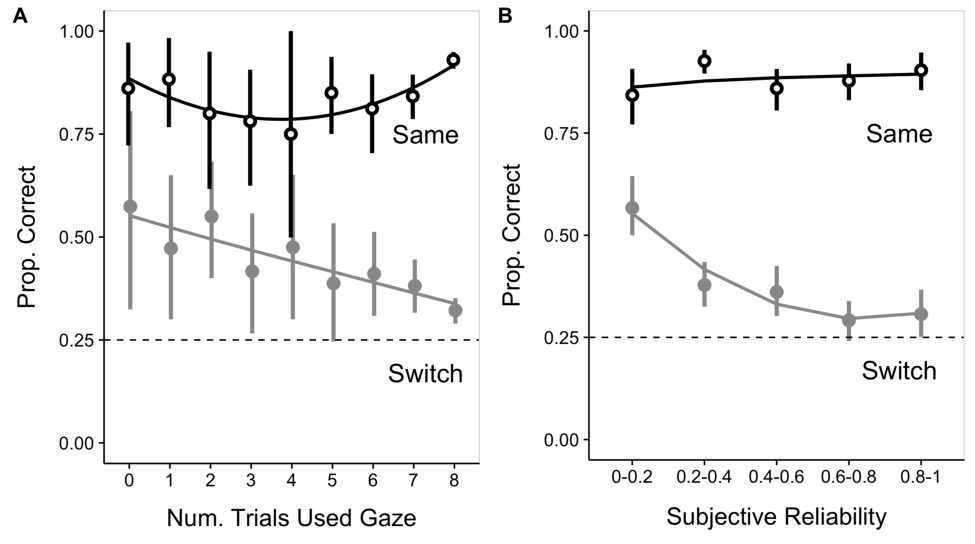
\includegraphics[width=0.9\linewidth]{figs/expt3-sub-plots-1} 

}

\caption[Secondary analyses of test trial performance in Experiment 3]{Secondary analyses of test trial performance in Experiment 3. Panel A shows accuracy as a function of the number of exposure trials on which participants chose to use the gaze cue. Panel B shows accuracy as a function of participants' subjective reliability judgments. The horizontal dashed lines represent chance performance, and error bars indicate 95\% confidence intervals computed by non-parametric bootstrap.}\label{fig:expt3-sub-plots}
\end{figure}
\end{CodeChunk}

\paragraph{Reliability condition
analysis}\label{reliability-condition-analysis}

To test the effect of reliability, we fit a model predicting accuracy at
test using reliability condition and test trial type as predictors. We
found a significant main effect of trial type (\(\beta = -3.95\), p
\textless{} .001), with lower accuracy on Switch trials. We also found
the key interaction between reliability condition and trial type
(\(\beta\) = -0.76, \(p\) = 0.044), such that when gaze was more
reliable, participants performed worse on Switch trials (see Panel A of
Figure 4). This interaction suggests that people stored more word-object
links as the learning context becomes more ambiguous. However, the
interaction between reliability and trial type was not particularly
strong, and -- similar to Experiment 1 -- there was variability in
performance across conditions (see the 50\% reliable condition in Panel
A of Figure 4). So to provide additional support for our hypothesis, we
conducted three follow-up analyses.

\paragraph{Gaze use analyses}\label{gaze-use-analyses}

We would only expect to see a strong interaction between reliability and
trial type if learners chose to use the gaze cue during exposure trials.
To test this hypothesis, we fit two additional models that included two
different measures of participants' use of the gaze cue. First, we added
accuracy on exposure trials as a predictor in our model. (Recall that
correct performance on exposure trials was defined as using the gaze
cue.) We found a significant interaction between accuracy on exposure
trials and trial type (\(\beta = -1.43\), \(p\) \textless{} .001) with
worse performance on Switch test trials when participants used gaze on
exposure trials (see Panel B of Figure 4). We also found an interaction
between gaze use and reliability (\(\beta = 0.97\), \(p\) = 0.004), such
that when gaze was more reliable, participants were more likely to use
it. The interaction between trial type and reliability became marginally
significant in this model (\(\beta = -0.62\), \(p\) = 0.086), suggesting
that \emph{use} of the gaze cue was a stronger predictor of memory for
alternative word-object links.
\footnote{We are grateful to an anonymous reviewer for suggesting this analysis, but we would like to note that it is an exploratory analysis.}

We also hypothesized that the reliability manipulation might change how
often individual participants chose to use the gaze cue throughout the
task. To explore this possibility, we fit a model with the same
specifications, but we included a predictor that we created by binning
participants based on the number of exposure trials on which they chose
to follow gaze (i.e., a gaze following score). We found a significant
interaction between how often participants chose to follow gaze on
exposure trials and trial type (\(\beta = -0.32\), p \textless{} .001),
such that participants who were more likely to use the gaze cue
performed worse on Switch trials, but not Same trials (see Panel A of
Figure 5).\footnote{We found this interaction while performing
  exploratory data analysis on a previous version of this study with an
  independent sample (N = 250, \(\beta = -0.29\), p \textless{} .001).
  The results reported here are from a separate sample where testing
  this interaction was a planned analysis.} Taken together, the two
analyses of participants' use of the gaze cue provide converging
evidence that when the speaker's gaze was reliable participants tended
to use the cue, and when they followed gaze, they tended to store less
information from the initial learning episode.

\paragraph{Subjective reliability
analysis}\label{subjective-reliability-analysis}

The strong interaction between use of the gaze cue and memory for
alternative word-object links suggests that participants' subjective
experience of reliability in the experiment mattered. Thus, we fit the
same model but substituted subjective reliability for the frequency of
gaze use as a predictor of test trial performance. We found a
significant interaction between trial type and participants' subjective
reliability assessments (\(\beta = -1.63\), p = 0.01): when participants
thought the speaker was more reliable, they performed worse on Switch
trials, but not Same trials (see Panel B of Figure 5).

\paragraph{Inspection time analyses}\label{inspection-time-analyses}

Finally, we were curious about how inspection time on exposure trials
affected accuracy at test. So we fit a model using inspection time and
trial type to predict accuracy and found a main effect of inspection
time (\(\beta\) = 0.22, \(p\) = 0.006), with longer inspection times
leading to better performance. The interaction between trial type and
inspection time was not significant, meaning that increased inspection
time had the same, positive effect on both Same and Switch trials. Next,
we explored the factors that influenced inspection time on exposure
trials by fitting a model to predict inspection time using reliability
and use of the gaze cue as predictors. We found a main effect of using
the gaze cue (-0.32, \(p\) \textless{} .001) with shorter inspection
times when participants chose to follow gaze. The main effect of
reliability condition and the interaction between reliability and use of
gaze were not significant. These analyses provide evidence that
\emph{use} of the gaze cue was the primary factor affecting how long
participants inspected the objects on exposure trials.

Together, these four analyses showed that when the speaker's gaze was
more reliable, participants were more likely to: (a) use the gaze cue,
(b) rate the speaker as more reliable, and (c) store fewer word-object
links, showing behavior more consistent with single hypothesis tracking.
These findings support and extend the results of Experiments 1 and 2 in
several important ways. First, participants' performance on Same trials
was again relatively unaffected by changes in performance on Switch
trials. The selective effect of gaze on Switch trials provides
converging evidence that the limitations on Same trials may be different
than those regulating the distribution of attention on Switch trials.
Second, learners' use of a referential cue was a stronger predictor of
reduced memory for alternative word-object links compared to our
reliability manipulation. Although we found a significant effect of
reliability on participants' use of the gaze cue, participants' tendency
to use the cue remained high. Consider that even in the 0\% reliability
condition the mean proportion of gaze following was still 0.82. It is
reasonable that participants would continue to use the gaze cue in our
experiment since it was the only cue available and participants did not
have a strong reason to think that the speaker would be deceptive.

The critical contribution of Experiment 3 is to show that learners
respond to a graded manipulation of referential uncertainty, with the
amount of information stored from the initial exposure tracking with the
reliability of the cue. This graded accuracy performance shows that
learners stored alternative word-object links with different levels of
fidelity depending on the amount of referential uncertainty present
during learning.

Across Experiments 1-3, learners tended to store fewer word-object links
in unambiguous learning contexts when a clear referential cue was
present. However, in all three experiments, participants' responses on
exposure trials controlled the length of the trial, which meant that
when participants used the gaze cue, they also spent less time visually
inspecting the objects. Thus, we do not know whether there is an
independent effect of referential cues on learners' underlying
representations, or if the effects found in Experiments 1-3 are entirely
mediated by a reduction in inspection time. In Experiment 4, we
addressed this possibility by removing participants' control over the
length of exposure trials, which made the inspection times on exposure
trials equivalent across the Gaze and No-Gaze conditions.

\section{Experiment 4}\label{experiment-4}

In Experiment 4, we asked whether less visual inspection time in the
gaze conditions can completely explain the effect of social cues on
learners' reduced memory for alternative word-object links. To answer
this question, we modified our paradigm and made the length of exposure
trials equivalent across the Gaze and No-Gaze conditions. In this
version of the task, participants saw the objects for a fixed amount of
time regardless of whether gaze was present. We also included two
different time windows for exposure trials in order to test whether gaze
would have a differential effect on shorter vs.~longer inspection times.
If the presence of gaze reduces learners' memory for multiple
word-object links, then this provides evidence that referential cues
affected the underlying representations over and above a reduction in
inspection time.

\begin{CodeChunk}
\begin{figure}[tb]

{\centering 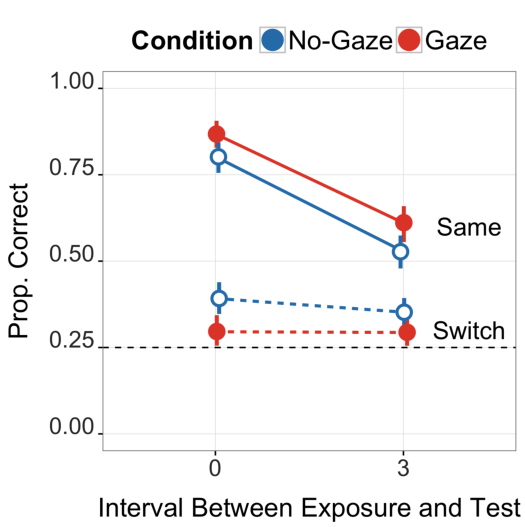
\includegraphics[width=0.5\linewidth]{figs/expt4-plot-1} 

}

\caption[Experiment 4 results]{Experiment 4 results. Accuracy on test trials in Experiment 4 collapsed across the Long and Short inspection time conditions. The dashed line represents chance performance. Color and line type indicate whether there was gaze present on exposure trials. Error bars indicate 95\% confidence intervals computed by non-parametric bootstrap. }\label{fig:expt4-plot}
\end{figure}
\end{CodeChunk}

\subsection{Method}\label{method-3}

\subsubsection{Participants}\label{participants-3}

Participant recruitment and inclusionary/exclusionary criteria were
identical to those of Experiments 1, 2, and 3. 100 HITs were posted for
each condition (1 Referent X 2 Intervals X 2 Inspection Time conditions)
for total of 400 paid HITs (excluded 37 HITs).

\subsubsection{Stimuli}\label{stimuli-2}

Audio, picture, and video stimuli were identical to Experiments 2 and 3.
Since inspection times were fixed across conditions, we wanted to ensure
that participants were aware of the time remaining on each exposure
trial. So we included a circular countdown timer located above the
center video. The timer remained on the screen during test trials but
did not count down since participants could take as much time as they
wanted to respond on test trials.

\subsubsection{Design and Procedure}\label{design-and-procedure-3}

Procedures were identical to those of Experiment 1-3. The design was
identical to that of Experiment 2 and consisted of 32 trials split into
2 blocks of 16 trials. Each block consisted of 8 exposure trials and 8
test trials (4 Same trials and 4 Switch trials) and contained only Gaze
or No-Gaze exposure trials. The order of block was counterbalanced
across participants.

The major design change was to make the length of exposure trials
equivalent across the Gaze and No-Gaze conditions. We randomly assigned
participants to one of two inspection time conditions: Short (6 seconds)
or Long (9 seconds). These times were selected based on participants'
self-paced inspection times in the Gaze and No-Gaze conditions in
Experiment 2. After pilot testing, we added three seconds to each
condition to ensure that participants had enough time to respond before
the experiment advanced. If participants did not respond in the allotted
time, an error message appeared informing participants that time had run
out and encouraged them to respond within the time window on subsequent
trials.

\subsection{Results and Discussion}\label{results-and-discussion-3}

We did not see strong evidence of an effect of the different inspection
times. Thus, all of the results reported here collapse across the short
and long inspection time conditions. For all analyses, we removed the
trials on which participants did not respond within the fixed inspection
time on exposure trials (0.05\% of trials).

\subsubsection{Exposure Trials}\label{exposure-trials-3}

Participants' responses on exposure trials differed from those expected
by chance (smallest \(\beta\) = 2.95, z = 38.08, p \textless{} .001),
suggesting that gaze was again effective in directing participants'
attention. Similar to Experiment 2, participants were quite likely to
use the gaze cue when it was a live actress (\(M_{0-interval}\) = 0.93,
\(M_{3-interval}\) = 0.95).

\subsubsection{Test Trials}\label{test-trials-3}

Figure 6 shows performance on test trials in Experiment 4. In the
majority of conditions, participants selected the correct referent at
rates greater than chance (smallest \(\beta\) = 0.2, z = 2.2, p
\textless{} .05). However, participants' responses were only marginally
different from chance on Switch trials after exposure trials with gaze
in the 3-interval condition (\(\beta\) = 0.17, \(p\) = 0.06).

We replicate the key finding from Experiments 1-3: after seeing exposure
trials with gaze, participants were less accurate on Switch trials
(\(\beta\) = 0.905, \(p\) \textless{} .001). Since inspection times were
fixed across the Gaze and No-Gaze conditions, this finding provides
evidence that the presence of a referential cue did more than just
reduce the amount of time participants' spent inspecting the potential
word-object links. In contrast to Experiments 1-3, visual inspection of
Figure 6 suggested that the referential cue provided a boost to accuracy
on Same trials. To assess the simple effects of gaze on trial type, we
computed pairwise contrasts using the \emph{lsmeans} package in R with a
Bonferroni correction for multiple comparisons (Lenth, 2016). Accuracy
was higher for Same trials in the Gaze condition (\(\beta\) = 0.49,
\(p\) \textless{} .001), and lower in the No-Gaze condition (\(\beta\) =
-0.41, \(p\) \textless{} .001). The boost in accuracy on Same trials
differs from Experiments 1-3 and suggests that making inspection times
equivalent across conditions allowed the social cue to affect the
strength of learners' memory for their candidate hypothesis.

The results of Experiment 4 help to clarify how gaze modulates memory in
our task, providing evidence that the presence of a referential cue does
more than just reduce participants' visual inspection time; instead, the
presence of gaze reduced memory for alternative word-object links even
when people had spent the same amount of time encoding the objects. We
also found evidence of a boost for learners' memory of their candidate
hypothesis in the gaze condition; an effect that we did not find in
Experiments 1-3. One explanation for this difference is that in
Experiment 4 participants' use of gaze was independent of the length of
exposure trials, which made inspection times in the gaze condition
longer compared to those in Experiments 1-3. Thus, it could be that the
combination of gaze with longer inspection times leads to a boost in
performance on Same trials relative to learning without gaze.

\section{General Discussion}\label{general-discussion}

Tracking cross-situational word-object statistics allows word learning
to proceed despite the presence of individually ambiguous naming events.
But models of cross-situational learning disagree about how much
information is actually stored in memory, and the input to statistical
learning mechanisms can vary along a continuum of referential
uncertainty. In the current line of work, we explore the hypothesis that
these two factors are fundamentally linked to one another and to the
social context in which word learning occurs. Specifically, we ask how
cross-situational learning operates over social input that modulates the
amount of ambiguity in the each learning context.

Our results suggest that the representations underlying
cross-situational learning are quite flexible. In the absence of a
referential cue to word meaning, people tended to store more alternative
word-object links. In contrast, when gaze was present learners stored
less information, showing behavior consistent with tracking a single
hypothesis (Experiments 1 and 2). Learners were also sensitive to a
parametric manipulation of the strength of the referential cue, showing
a graded increase in the tendency to use the cue as reliability
increased, which in turn resulted in a graded decrease in memory for
alternative word-object links (Experiment 3). Finally, learners stored
less information in the presence of gaze even when they spent the same
amount of time visually inspecting the objects during learning
(Experiment 4).

In Experiments 1-3, reduced memory for alternative hypotheses did not
result in a boost to memory for learners' candidate hypothesis. This
pattern of data suggests that the presence of a referential cue
selectively affected one component of the underlying representation: the
number of alternative word-object links, and not learners' initial
candidate hypothesis. However, when the length of exposure trials was
made equivalent across the gaze conditions in Experiment 4, learners
showed stronger memory for their initial hypothesis when gaze was
present. This suggests that the relationship between referential cues
and the strength of learners' candidate hypothesis is modulated by how
the cue interacts with visual inspection time: when coupled with longer
inspection times, gaze provided a boost to memory.

\subsection{Relationship to previous
work}\label{relationship-to-previous-work}

Why did we not see an increase in the strength of learners' candidate
hypothesis in Experiments 1-3? One possibility is that participants did
not shift their cognitive resources from the set of alternatives to
their single hypothesis, but instead rationally conserved their
resources for future use. Griffiths, Lieder, and Goodman (2015)
formalize this behavior by pushing the rationality of
computational-level models down to the psychological process level. In
their framework, cognitive systems are thought to be adaptive in that
they optimize the use of their limited resources, taking the cost of
computation (e.g., the opportunity cost of time or mental opportunity)
into account. For example, Vul, Goodman, Griffiths, and Tenenbaum (2014)
showed that as time pressure increased in a decision-making task,
participants were more likely to show behavior consistent with a less
cognitively challenging strategy of matching, rather than with the
globally optimal strategy. In the current work, we found that learners
showed evidence of altering how they allocated cognitive resources based
on the amount of referential uncertainty present during learning,
spending less time inspecting alternative word-object links and reducing
the number of links stored in memory when uncertainty was low.

Our results also fit well with recent experimental work that
investigates how attention and memory can constrain infants' statistical
word learning. For example, Smith and Yu (2013) used a modified
cross-situational learning task to show that only infants who disengaged
from a novel object to look at both potential referents were able to
learn the correct word--object mappings. Moreover, Vlach and Johnson
(2013) showed that 16-month-olds were only able to learn from adjacent
cross-situational co-occurrence statistics, and unable to learn from
co-occurrences that were separated in time. Both of these findings make
the important point that only the information that comes into contact
with the learning system can be used for cross-situational word
learning, and this information is directly influenced by the attention
and memory constraints of the learner.

Moreover, these results add to a large literature showing the importance
of social information for word learning (P. Bloom, 2002; Clark, 2009;
Hollich et al., 2000). These findings also bring Social-pragmatic
theories of language acquisition into contact with studies exploring the
interaction between statistical learning and other types of cues (Frank,
Goodman, \& Tenenbaum, 2009; Yu \& Ballard, 2007). For example, Yoshida,
Rhemtulla, and Vouloumanos (2012) showed that in an associative learning
task, adults only use exclusion learning processes (i.e., discarding
known alternatives) with speech, and not for nonspeech labels,
suggesting that adults constrained learning differently depending on the
type of stimuli. Our findings suggest that referential cues present in
the social context interact with statistical learning by modulating the
amount of information that is stored in the underlying representations
that support learning over time.

But how should we characterize the effect of gaze on attention and
memory in our task? One possibility is that the referential cue acts as
a filter, only allowing likely referents to contact statistical learning
mechanisms (Yu \& Ballard, 2007). This `filtering account' separates the
effect of social cues from the underlying computation that aggregates
cross-situational information. Another possibility is that referential
cues provide evidence about a speaker's communicative intent (Frank et
al., 2009). In this model, the learner is reasoning about the speaker
and word meanings simultaneously, which places inferences based on
social information as part of the underlying computation. A third
possibility is that participants thought of the referential cue as
pedagogical. In this context, learners assume that the speaker will
choose an action that is most likely to increase the learner's belief in
the true state of the world (Shafto, Goodman, \& Frank, 2012), making it
unnecessary to allocate resources to alternative hypotheses. Experiments
show that children spend less time exploring an object and are less
likely to discover alternative object-functions if a single function is
demonstrated in a pedagogical context (Bonawitz et al., 2011). However,
because the results from the current study cannot distinguish between
these explanations, these questions remain topics for future studies
specifically designed to tease apart these possibilities.

Is gaze a privileged cue, or could other, perhaps less-social cues
(e.g., an arrow) also modulate the representations underlying
cross-situational learning? On the one hand, previous research suggests
that gaze cues lead to more reflexive attentional responses compared to
arrows (Friesen, Ristic, \& Kingstone, 2004), that gaze-triggered
attention results in better learning compared to salience-triggered
attention (e.g., via flashing objects) (Wu \& Kirkham, 2010), and that
even toddlers readily use gaze to infer novel word meanings (Baldwin,
1993). Thus, it could be that gaze is an especially effective cue for
constraining word learning since it often communicates a speaker's
referential intent and is a particularly powerful way to guide
attention. On the other hand, the generative process of the cue (i.e.,
whether it is more or less social) might be less important; instead, the
critical factor might be whether the cue effectively reduces referential
uncertainty during the initial learning episode. Future work could
explore a wider range of cues (e.g., pointing or object salience) to see
if they modulate the representations underlying cross-situational
learning in a similar way.

\subsection{Limitations}\label{limitations}

There are several limitations to the current study that are worth
noting. First, the social context that we used was relatively
impoverished. Although we moved beyond a simple manipulation of the
presence or absence of social information, we isolated just a single cue
to reference, gaze. But real-world learning contexts are much more
complex, providing learners access to multiple cues such as gaze,
pointing, and previous discourse. In fact, Frank, Tenenbaum, and Fernald
(2013) analyzed a corpus of parent-child interactions and concluded that
learners would do better to aggregate noisy social information from
multiple cues, rather than monitor a single cue since no single cue was
a consistent predictor of reference. In our data, we did see a more
reliable effect of referential cues when we used a live actress, which
included both gaze and head turn as opposed to the static, schematic
stimuli, which only included gaze. It is still an open and interesting
question as to how our results would generalize to learning environments
that contain a rich combination of social cues.

Second, we do not yet know how variations in referential uncertainty
during learning might affect the representations of young word learners.
Recent research using a similar paradigm did not find evidence that 2-
or 3-year-olds store multiple word-object links; instead, children only
retained a single candidate hypothesis (Woodard, Gleitman, \& Trueswell,
2016). However, performance limitations on children's developing visual
attention and memory systems (Colombo, 2001; Ross-sheehy, Oakes, \&
Luck, 2003) could make success on explicit response tasks such as these
difficult. Thus, we think that it will be important to test a variety of
outcome measures to see if young learners show evidence of storing
multiple word meanings during learning. Moreover, previous work with
infants has shown that their attention is often stimulus-driven and
sticky (Oakes, 2011), suggesting that very young word learners might not
effectively explore the visual scene in order to extract the necessary
statistics for storing multiple alternatives. It could be that
referential cues play an even more important role for young learners by
filtering the input to cross-situational word learning mechanisms and
guiding them to the relevant statistics in the input. In fact, recent
work has shown that the precise timing of features such as increased
parent attention and gesturing towards a named object and away from
non-target objects were strong predictors of the referential clarity of
a naming event (Trueswell et al., 2016). It could be that the statistics
available in these particularly clear naming events are the most useful
for young learners to retain for cross-situational learning.

Finally, the current experiments used a restricted cross-situational
word learning scenario, which differs from real-world language learning
contexts in several important ways. One, we only tested a single
exposure for each novel word-object pairing; whereas, real-world naming
events are best characterized by discourse where an object is likely to
be named repeatedly in a short amount of time (Frank, Tenenbaum, \&
Fernald, 2013; Rohde \& Frank, 2014). Two, the restricted visual world
of 2-8 objects on a screen combined with the forced-choice response
format may have biased people to assume that all words in the task must
have referred to one of the objects on the screen. But, in actual
language usage people can refer to things that are not physically
co-present (e.g., L. Gleitman, 1990), creating a scenario where learners
would not benefit from storing additional word-object links in the
absence of clear referential cues. Finally, we presented novel words in
isolation, removing any sentential cues to word meaning (e.g.,
verb-argument relations). Previous work shows that sentence-level
constraints interact with cross-situational word learning mechanisms
(Koehne \& Crocker, 2014). Thus, we need more evidence to understand how
the representations underlying cross-situational learning change in
response to referential uncertainty at different timescales and in
richer language contexts that more accurately reflect real-world
learning environments.

\subsection{Conclusions}\label{conclusions}

Word learning proceeds despite the potential for high levels of
referential uncertainty and despite learners' limited cognitive
resources. Our work shows that cross-situational learners flexibly
respond to the amount of ambiguity in the input, and as referential
uncertainty increases, learners tended to store more word-object links.
Overall, these results bring together aspects of social and statistical
accounts of word learning to increase our understanding of how social
information modulates the input to statistical learning mechanisms.

\newpage

\section{Acknowledgements}\label{acknowledgements}

We are grateful to Rose Schneider for helping record stimuli and to the
members of the Language and Cognition Lab for their feedback on this
project. This work was supported by a National Science Foundation
Graduate Research Fellowship to KM, an NIH NRSA Postdoctoral Fellowship
to DY, and a John Merck Scholars Fellowship to M.C.F.

\newpage

\section{References}\label{references}

\setlength{\parindent}{-0.1in} \setlength{\leftskip}{0.125in} \noindent

\hypertarget{refs}{}
\hypertarget{ref-baldwin1993infants}{}
Baldwin, D. A. (1993). Infants' ability to consult the speaker for clues
to word reference. \emph{Journal of Child Language}, \emph{20}(02),
395--418.

\hypertarget{ref-bates2013lme4}{}
Bates, D., Maechler, M., Bolker, B., \& Walker, S. (2013). Lme4: Linear
mixed-effects models using eigen and s4. \emph{R Package Version},
\emph{1}(4).

\hypertarget{ref-bloom2002children}{}
Bloom, P. (2002). \emph{How children learn the meaning of words}. The
MIT Press.

\hypertarget{ref-bonawitz2011double}{}
Bonawitz, E., Shafto, P., Gweon, H., Goodman, N. D., Spelke, E., \&
Schulz, L. (2011). The double-edged sword of pedagogy: Instruction
limits spontaneous exploration and discovery. \emph{Cognition},
\emph{120}(3), 322--330.

\hypertarget{ref-brooks2005development}{}
Brooks, R., \& Meltzoff, A. N. (2005). The development of gaze following
and its relation to language. \emph{Developmental Science}, \emph{8}(6),
535--543.

\hypertarget{ref-brooks2008infant}{}
Brooks, R., \& Meltzoff, A. N. (2008). Infant gaze following and
pointing predict accelerated vocabulary growth through two years of age:
A longitudinal, growth curve modeling study. \emph{Journal of Child
Language}, \emph{35}(01), 207--220.

\hypertarget{ref-carpenter1998social}{}
Carpenter, M., Nagell, K., Tomasello, M., Butterworth, G., \& Moore, C.
(1998). Social cognition, joint attention, and communicative competence
from 9 to 15 months of age. \emph{Monographs of the Society for Research
in Child Development}, i--174.

\hypertarget{ref-cartmill2013quality}{}
Cartmill, E. A., Armstrong, B. F., Gleitman, L. R., Goldin-Meadow, S.,
Medina, T. N., \& Trueswell, J. C. (2013). Quality of early parent input
predicts child vocabulary 3 years later. \emph{Proceedings of the
National Academy of Sciences}, \emph{110}(28), 11278--11283.

\hypertarget{ref-clark2009first}{}
Clark, E. V. (2009). \emph{First language acquisition}. Cambridge
University Press.

\hypertarget{ref-cleveland2007joint}{}
Cleveland, A., Schug, M., \& Striano, T. (2007). Joint attention and
object learning in 5-and 7-month-old infants. \emph{Infant and Child
Development}, \emph{16}(3), 295--306.

\hypertarget{ref-colombo2001development}{}
Colombo, J. (2001). The development of visual attention in infancy.
\emph{Annual Review of Psychology}, \emph{52}(1), 337--367.

\hypertarget{ref-frank2009using}{}
Frank, M. C., Goodman, N. D., \& Tenenbaum, J. B. (2009). Using
speakers' referential intentions to model early cross-situational word
learning. \emph{Psychological Science}, \emph{20}(5), 578--585.

\hypertarget{ref-frank2013social}{}
Frank, M. C., Tenenbaum, J. B., \& Fernald, A. (2013). Social and
discourse contributions to the determination of reference in
cross-situational word learning. \emph{Language Learning and
Development}, \emph{9}(1), 1--24.

\hypertarget{ref-friesen2004attentional}{}
Friesen, C. K., Ristic, J., \& Kingstone, A. (2004). Attentional effects
of counterpredictive gaze and arrow cues. \emph{Journal of Experimental
Psychology: Human Perception and Performance}, \emph{30}(2), 319.

\hypertarget{ref-gleitman1990structural}{}
Gleitman, L. (1990). The structural sources of verb meanings.
\emph{Language Acquisition}, \emph{1}(1), 3--55.

\hypertarget{ref-griffiths2015rational}{}
Griffiths, T. L., Lieder, F., \& Goodman, N. D. (2015). Rational use of
cognitive resources: Levels of analysis between the computational and
the algorithmic. \emph{Topics in Cognitive Science}, \emph{7}(2),
217--229.

\hypertarget{ref-hollich2000breaking}{}
Hollich, G. J., Hirsh-Pasek, K., Golinkoff, R. M., Brand, R. J., Brown,
E., Chung, H. L., \ldots{} Bloom, L. (2000). Breaking the language
barrier: An emergentist coalition model for the origins of word
learning. \emph{Monographs of the Society for Research in Child
Development}, i--135.

\hypertarget{ref-kanwisher1997locus}{}
Kanwisher, N., Woods, R. P., Iacoboni, M., \& Mazziotta, J. C. (1997). A
locus in human extrastriate cortex for visual shape analysis.
\emph{Journal of Cognitive Neuroscience}, \emph{9}(1), 133--142.

\hypertarget{ref-koehne2014interplay}{}
Koehne, J., \& Crocker, M. W. (2014). The interplay of cross-situational
word learning and sentence-level constraints. \emph{Cognitive Science}.

\hypertarget{ref-koenig2004trust}{}
Koenig, M. A., Clement, F., \& Harris, P. L. (2004). Trust in testimony:
Children's use of true and false statements. \emph{Psychological
Science}, \emph{15}(10), 694--698.

\hypertarget{ref-lenth2016lsmeans}{}
Lenth, R. V. (2016). Least-squares means: The R package lsmeans.
\emph{Journal of Statistical Software}, \emph{69}(1), 1--33.
\url{http://doi.org/10.18637/jss.v069.i01}

\hypertarget{ref-mcmurray2012word}{}
McMurray, B., Horst, J. S., \& Samuelson, L. K. (2012). Word learning
emerges from the interaction of online referent selection and slow
associative learning. \emph{Psychological Review}, \emph{119}(4), 831.

\hypertarget{ref-medina2011words}{}
Medina, T. N., Snedeker, J., Trueswell, J. C., \& Gleitman, L. R.
(2011). How words can and cannot be learned by observation.
\emph{Proceedings of the National Academy of Sciences}, \emph{108}(22),
9014--9019.

\hypertarget{ref-oakes2011infant}{}
Oakes, L. M. (2011). \emph{Infant perception and cognition: Recent
advances, emerging theories, and future directions}. Oxford University
Press, USA.

\hypertarget{ref-quine19600}{}
Quine, W. V. (1960). 0. word and object. \emph{111e MIT Press}.

\hypertarget{ref-rohde2014markers}{}
Rohde, H., \& Frank, M. C. (2014). Markers of topical discourse in
child-directed speech. \emph{Cognitive Science}, \emph{38}(8),
1634--1661.

\hypertarget{ref-ross2003development}{}
Ross-sheehy, S., Oakes, L. M., \& Luck, S. J. (2003). The development of
visual short-term memory capacity in infants. \emph{Child Development},
\emph{74}(6), 1807--1822.

\hypertarget{ref-shafto2012learning}{}
Shafto, P., Goodman, N. D., \& Frank, M. C. (2012). Learning from others
the consequences of psychological reasoning for human learning.
\emph{Perspectives on Psychological Science}, \emph{7}(4), 341--351.

\hypertarget{ref-siskind1996computational}{}
Siskind, J. M. (1996). A computational study of cross-situational
techniques for learning word-to-meaning mappings. \emph{Cognition},
\emph{61}(1), 39--91.

\hypertarget{ref-smith2011cross}{}
Smith, K., Smith, A. D., \& Blythe, R. A. (2011). Cross-situational
learning: An experimental study of word-learning mechanisms.
\emph{Cognitive Science}, \emph{35}(3), 480--498.

\hypertarget{ref-smith2008infants}{}
Smith, L. B., \& Yu, C. (2008). Infants rapidly learn word-referent
mappings via cross-situational statistics. \emph{Cognition},
\emph{106}(3), 1558--1568.

\hypertarget{ref-smith2013visual}{}
Smith, L. B., \& Yu, C. (2013). Visual attention is not enough:
Individual differences in statistical word-referent learning in infants.
\emph{Language Learning and Development}, \emph{9}(1), 25--49.

\hypertarget{ref-smith2014unrealized}{}
Smith, L. B., Suanda, S. H., \& Yu, C. (2014). The unrealized promise of
infant statistical word--referent learning. \emph{Trends in Cognitive
Sciences}, \emph{18}(5), 251--258.

\hypertarget{ref-trueswell2016perceiving}{}
Trueswell, J. C., Lin, Y., Armstrong, B., Cartmill, E. A.,
Goldin-Meadow, S., \& Gleitman, L. R. (2016). Perceiving referential
intent: Dynamics of reference in natural parent--child interactions.
\emph{Cognition}, \emph{148}, 117--135.

\hypertarget{ref-trueswell2013propose}{}
Trueswell, J. C., Medina, T. N., Hafri, A., \& Gleitman, L. R. (2013).
Propose but verify: Fast mapping meets cross-situational word learning.
\emph{Cognitive Psychology}, \emph{66}(1), 126--156.

\hypertarget{ref-vlach2013memory}{}
Vlach, H. A., \& Johnson, S. P. (2013). Memory constraints on infants'
cross-situational statistical learning. \emph{Cognition}, \emph{127}(3),
375--382.

\hypertarget{ref-vouloumanos2008fine}{}
Vouloumanos, A. (2008). Fine-grained sensitivity to statistical
information in adult word learning. \emph{Cognition}, \emph{107}(2),
729--742.

\hypertarget{ref-vul2014}{}
Vul, E., Goodman, N., Griffiths, T. L., \& Tenenbaum, J. B. (2014). One
and done? Optimal decisions from very few samples. \emph{Cognitive
Science}, \emph{38}(4), 599--637.

\hypertarget{ref-woodard2016two}{}
Woodard, K., Gleitman, L. R., \& Trueswell, J. C. (2016). Two-and
three-year-olds track a single meaning during word learning: Evidence
for propose-but-verify. \emph{Language Learning and Development},
\emph{12}(3), 252--261.

\hypertarget{ref-wu2010no}{}
Wu, R., \& Kirkham, N. Z. (2010). No two cues are alike: Depth of
learning during infancy is dependent on what orients attention.
\emph{Journal of Experimental Child Psychology}, \emph{107}(2),
118--136.

\hypertarget{ref-wu2011infants}{}
Wu, R., Gopnik, A., Richardson, D. C., \& Kirkham, N. Z. (2011). Infants
learn about objects from statistics and people. \emph{Developmental
Psychology}, \emph{47}(5), 1220.

\hypertarget{ref-yoon2008communication}{}
Yoon, J. M., Johnson, M. H., \& Csibra, G. (2008). Communication-induced
memory biases in preverbal infants. \emph{Proceedings of the National
Academy of Sciences}, \emph{105}(36), 13690--13695.

\hypertarget{ref-yoshida2012exclusion}{}
Yoshida, K., Rhemtulla, M., \& Vouloumanos, A. (2012). Exclusion
constraints facilitate statistical word learning. \emph{Cognitive
Science}, \emph{36}(5), 933--947.

\hypertarget{ref-yu2007unified}{}
Yu, C., \& Ballard, D. H. (2007). A unified model of early word
learning: Integrating statistical and social cues.
\emph{Neurocomputing}, \emph{70}(13), 2149--2165.

\hypertarget{ref-yu2007rapid}{}
Yu, C., \& Smith, L. B. (2007). Rapid word learning under uncertainty
via cross-situational statistics. \emph{Psychological Science},
\emph{18}(5), 414--420.

\hypertarget{ref-yu2012embodied}{}
Yu, C., \& Smith, L. B. (2012). Embodied attention and word learning by
toddlers. \emph{Cognition}.

\hypertarget{ref-yurovsky2014algorithmic}{}
Yurovsky, D., \& Frank, M. C. (2015). An integrative account of
constraints on cross-situational learning. \emph{Cognition}.

\hypertarget{ref-yurovsky2013statistical}{}
Yurovsky, D., Smith, L. B., \& Yu, C. (2013). Statistical word learning
at scale: The baby's view is better. \emph{Developmental Science},
\emph{16}(6), 959--966.

\bibliography{}

\end{document}
